% !TEX root = msc_thesis.tex

\chapter{Implementation} \label{ch:implementation}


\section{Profs} \label{sec:profs}

ELASPIC uses a domain-based approach for creating homology models of query proteins, and therefore requires access to accurate domain definitions. The most widely-used source of protein domain definitions is Pfam \cite{punta_pfam_2012}. However, since Pfam domains definitions are based entirely on protein sequence, they correlate poorly with the structural fold of the protein. Using Pfam domain definitions when making homology models tends to produce unstable models of fragmented and / or truncated domains, and this would compromise our subsequent analysis of the structural impact of mutations.

In order to improve the structural accuracy of Pfam domains, Andres Felipe Giraldo Forero developed a pipeline that uses structural alignments and a set of heuristics to modify Pfam domain definitions and make them better aligned with the tertiary structure of the protein, as defined by CATH \cite{cuff_extending_2011}. He named this pipeline Profs, for Protein families. A schematic of this pipeline is presented in Figure \ref{fig:profs_pipeline}, and an R package implementing the pipeline is available at \url{https://bitbucket.org/afgiraldofo/profs}. Profs domains have an advantage over Pfam domains in that they have been corrected and expanded to match the structural fold of the protein. They have an advantage over CATH domains in that they are backed by large, manually-seeded alignments, and can be easily detected in any protein sequence using Pfam HMMs.

We used Andres' pipeline to annotate with Profs domains all proteins in the UniProt database. The resulting table of Profs domain definitions is available for download from the ELASPIC website ( \url{http://elaspic.kimlab.org/static/download/}) and is included in the ELASPIC database (see \textbf{domain} and \textbf{domain\_contact} tables in Figure \ref{fig:elaspic_database_schema} and Table \ref{tab:elaspic_database_schema}). The following sections describe the procedure used to generate tables of Profs domain definitions and Profs domain-domain interactions that are used by ELASPIC.

\begin{figure}[t]
	\centering
	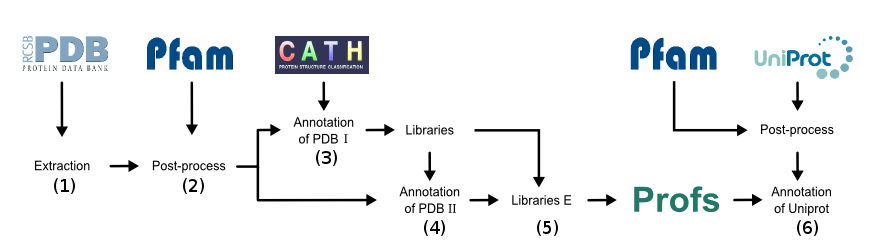
\includegraphics[width=1.0\linewidth]{static/profs/profs_pipeline.png}
	\caption[Profs pipeline.]{Flowchart illustrating steps in the Profs pipeline (courtesy of Andres Felipe Giraldo Forero). \textbf{(1)} All structures in the PDB are parsed to extract protein sequences, and \textit{hmmscan} is ran to find Pfam domains in those sequences. \textbf{(2)} Pfam domains of proteins in the PDB are processed in order to join and / or remove overlapping and repeating domains. \textbf{(3)} Pfam domain definitions are altered in order to make them compatible with CATH definitions, for structures that have been annotated by CATH. \textbf{(4)} Pfam domain definitions are altered in order to make them compatible with CATH definitions, for structures that have not been annotated by CATH. This is done by performing pairwise alignments with structures that do have CATH annotations. \textbf{(5)} Libraries of Profs domain definitions, and Profs domain-domain interactions, are generated for all proteins in the PDB.  \textbf{(6)} Libraries of Profs domain definitions, and Profs domain-domain interactions, are generated for all proteins in Uniprot.}
	\label{fig:profs_pipeline}
\end{figure}


\subsection{Domains}

We used Profs domain definitions, which had been calculated for all proteins in the PDB, to find Profs domains, and structural templates for those domains, for all proteins in UniProt (step 6 in Figure \ref{fig:profs_pipeline}). To do this, we followed the same procedure that was used by the authors of Profs to annotate structures in the PDB that have Pfam domains but no CATH domains \cite{witvliet_elaspic_2016}.

We started with Pfam domain definitions for all known protein sequences, which we download from the SIMAP website \cite{rattei_simapcomprehensive_2010}. We mapped those protein sequences to Uniprot using the MD5 hash of each sequence, and we joined or removed overlapping and repeating domains using a mapping table supplied with the Profs R package. Next, we tried to find a Profs structural template for each Pfam domain by running \textit{blastp} against libraries of Profs domains, which are included in the Profs R package. If a suitable template was found, we proceeded to do iterative global alignments using Muscle \cite{edgar_muscle:_2004} while expanding domain boundaries of the Pfam domains to match domain boundaries of the Profs templates. If two Pfam domains were expanded to occupy the same region in the protein, that region was divided in half and attached to the preceding and the succeeding domains.

The results of this analysis are stored in the \textbf{uniprot\_domain} and the \textbf{uniprot\_domain\_template} tables in the ELASPIC database (Figure \ref{fig:elaspic_database_schema}). The \textbf{uniprot\_domain} table contains all Pfam domains and supradomains that are obtained after removing repeating and overlapping domains, as outlined above. The \textit{pdbfam\_name} column contains the name of the Profs domain. The \textit{alignment\_def} column contains either the original Pfam domain definitions or, in the case of supradomains, the merged domain definitions of multiple Pfam domains. The \textbf{uniprot\_domain\_template} table contains information describing the alignment of the Pfam domain or supradomain with the corresponding Profs structural template, for domains for which a suitable Profs template could be found. The \textit{cath\_id} column identifies the Profs structural template that was selected, and the \textit{domain\_def} column contains the corrected and expanded domain definitions.


\subsection{Comparison with Pfam and Gene3D}

In order to ascertain the validity of Profs domain definitions, we compared Profs, Pfam and Gene3D in terms of sequence coverage (Figure \ref{fig:profs_coverage}) and domain size (Figure \ref{fig:profs_domain_size}).

We downloaded Pfam and Gene3D domain definitions for all human proteins from SIMAP \cite{rattei_simapcomprehensive_2010}, and we calculated Profs domain definitions following the pipeline described above. The analysis was restricted to 18,828 human proteins from UniProt which are annotated with at least one Profs, Pfam or Gene3D domain.

In order to compare sequence coverage, we looked at the fraction of all protein sequences which are covered by each domain type (Figure \ref{fig:profs_coverage}). Overall, Profs has the highest sequence coverage, with 55.7 \% of 10,868,810 amino acids in 18,828 proteins residing inside a Profs domain. Profs annotates $\approx$ 9\% more amino acids than Pfam and $\approx$ 14\% more amino acids than Gene3D, although the relatively low coverage by Gene3D is expected, as it can only detect domains which are represented in the PDB.

In order to compare domain size, we looked at the average number of domains per protein for each of the three methods (Figure \ref{fig:profs_domain_size}). Profs has more proteins with only one domain per protein, while Pfam and Gene3D have more proteins with two or more domains per protein. This is consistent with Profs trying to join fragmented and repeating domains into consistent structural units. Gene3D does not detect domains in many proteins with Profs and Pfam domains, likely because those domains have not been crystallized.

The result of this analysis shows that, at least for human proteins, Profs achieves higher sequence coverage using fewer domains per protein than either Pfam or Gene3D. This makes Profs well-suited for the ELASPIC pipeline.


\begin{figure}[!tb]
	\centering
	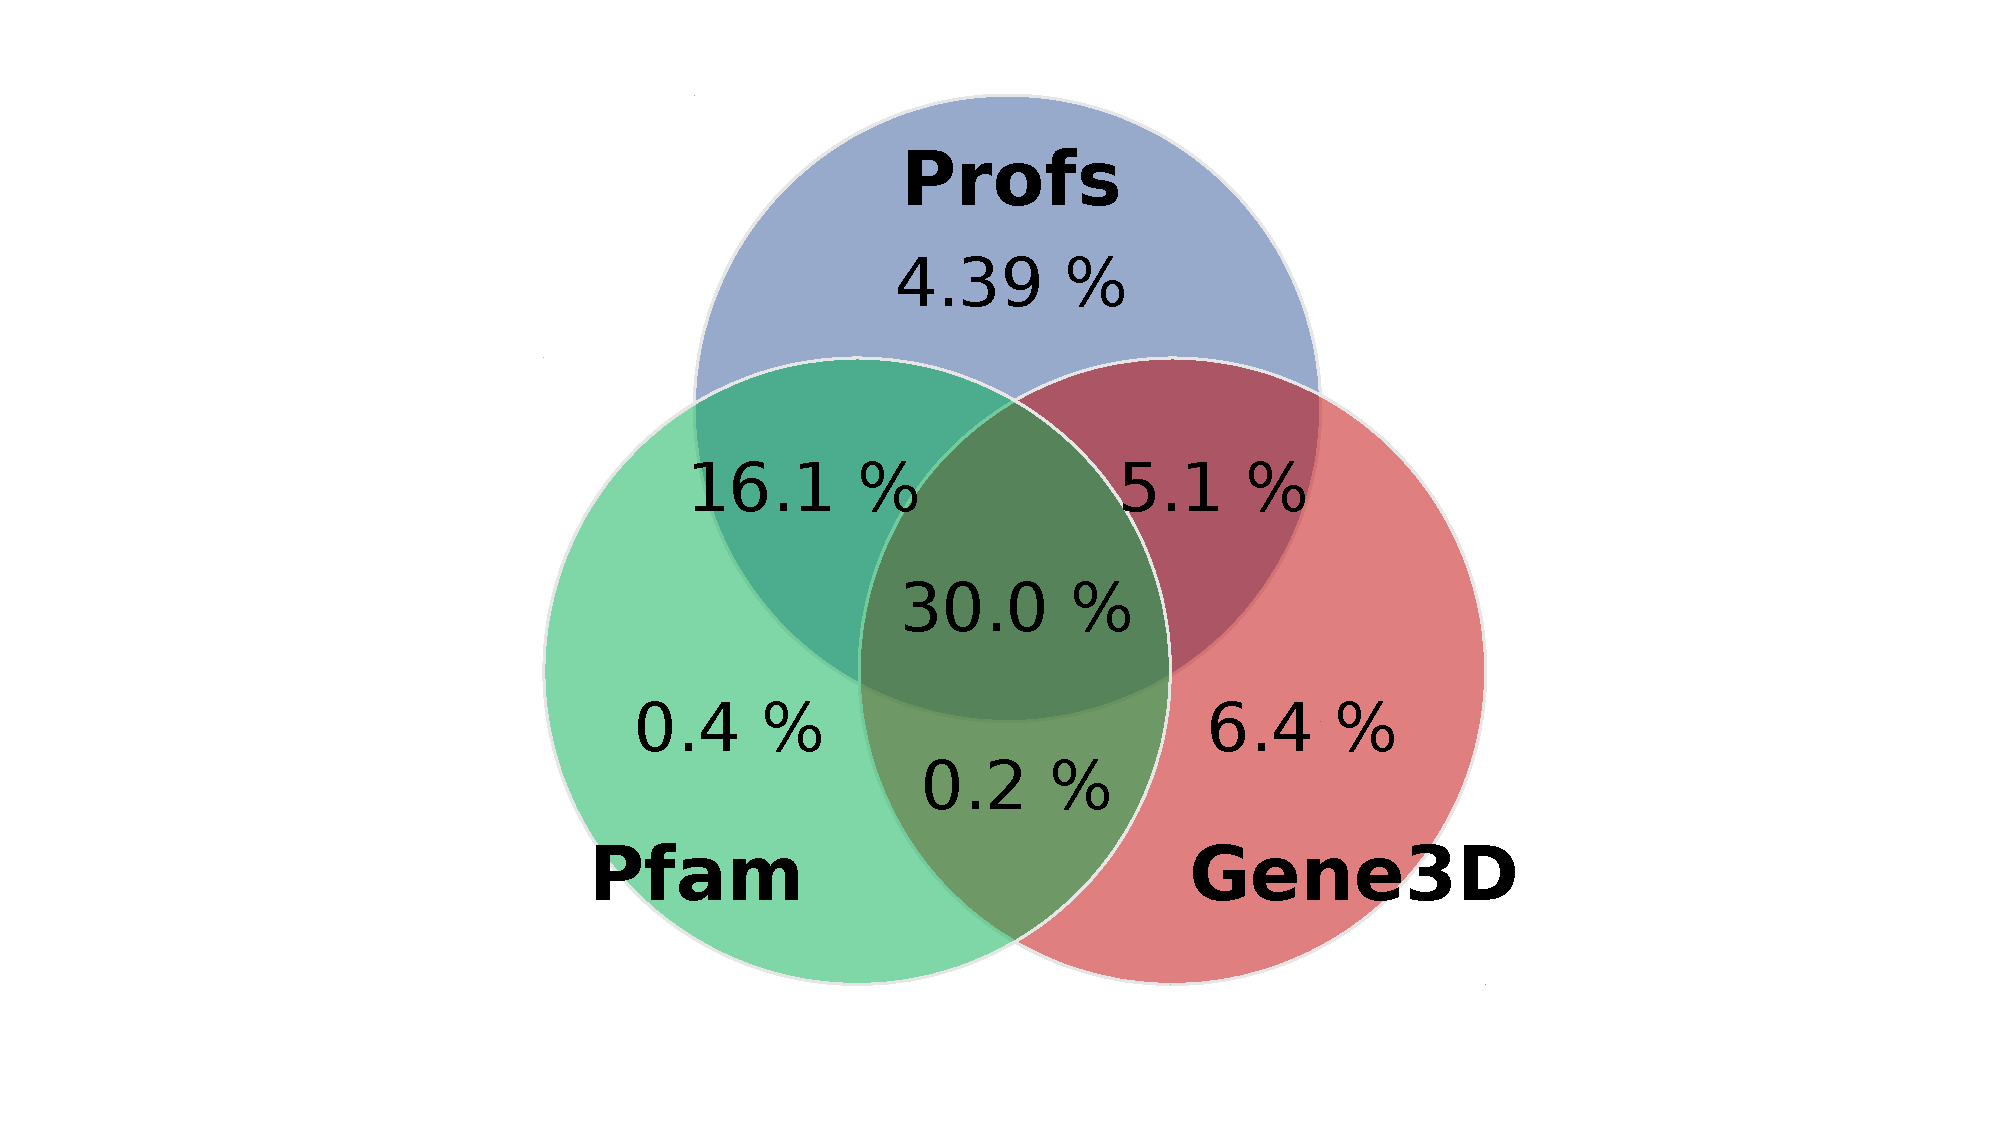
\includegraphics[width=0.7\textwidth]{static/profs/uniprot_coverage_statistics.pdf}
	\caption[Profs, Pfam, and Gene3D domain overlap.]{Venn diagram showing the overlap in domain definitions between Profs, Pfam, and Gene3D. Values represent the fraction of amino acids, of all human proteins in UniProt, which are covered by the particular domain or domains. A total of 18,828 human proteins and 10,868,810 amino acids were considered, after excluding proteins which had no predicted domains by any method. Profs has the highest coverage, with 55.7 \% of amino acids being annotated by a Prof domain.}
	\label{fig:profs_coverage}
\end{figure}


\begin{figure}[!tb]
	\centering
	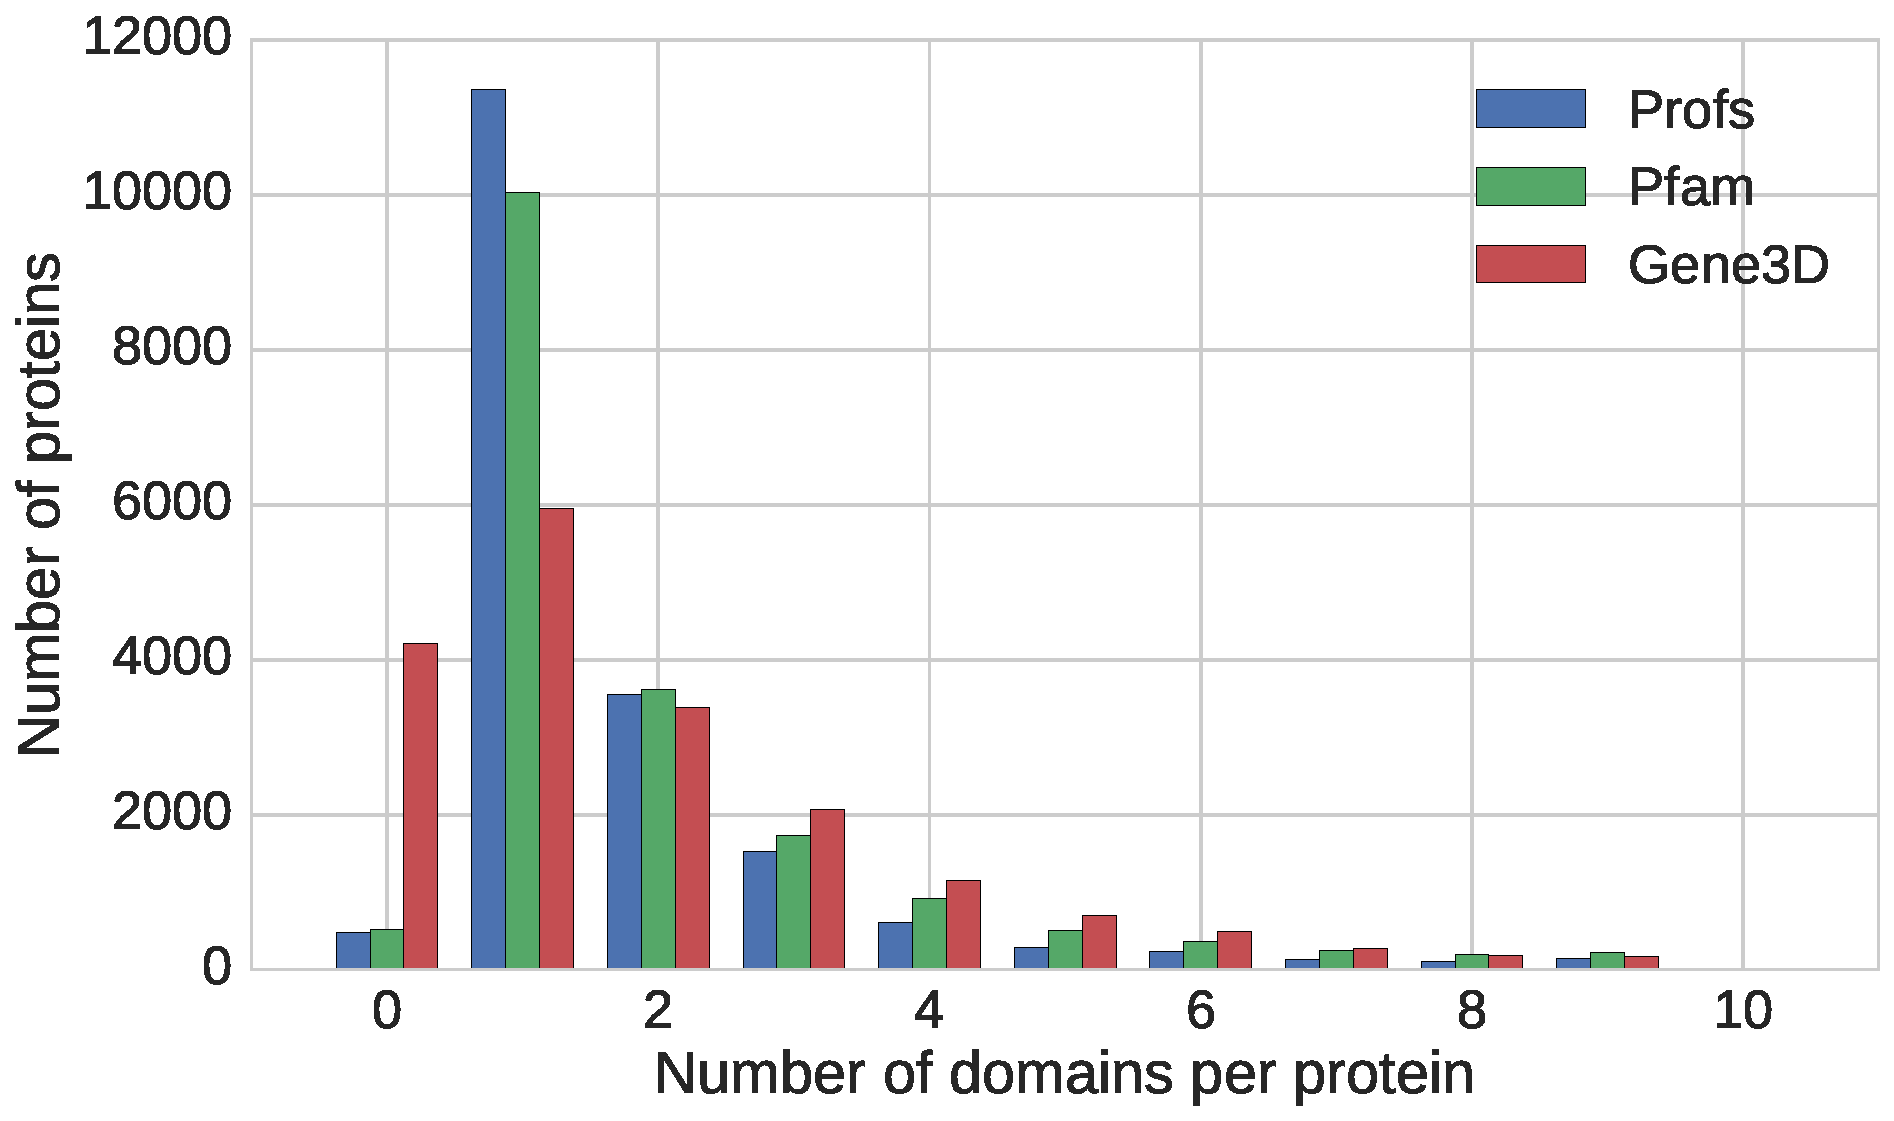
\includegraphics[width=0.9\textwidth]{static/profs/domains_per_protein.pdf}
	\caption[Profs, Pfam, and Gene3D domains per protein.]{Average number of Profs, Pfam and Gene3D domains per protein, for all human proteins containing at least one domains. Profs tends to have fewer domains per protein then either Pfam or Gene3D, even though Profs domains have higher sequence coverage (see Figure \ref{fig:profs_coverage}). Gene3D lacks domain annotation for many proteins which contain at least one Pfam and Profs domain.}
	\label{fig:profs_domain_size}
\end{figure}



\subsection{Domain interactions}

We also created a table of domain-domain interactions for proteins that are known to interact and for which a homology model of the interaction can be created. We started by creating a comprehensive list of protein-protein interactions (PPIs), by taking the union of all PPIs listed in the HIPPIE database \cite{schaefer_hippie:_2012} and in the datasets hosted by the Harvard Center for Cancer Systems Biology (CCSB) \cite{rolland_proteome-scale_2014}. The overlap in the PPIs obtained from each source is presented in Figure \ref{fig:ppi_database_overlap}. We filtered those PPIs to select pairs of proteins where each protein has at least one domain with a structural template. This information is stored in the \textbf{uniprot\_domain\_pair} table. For each of those domains, we perform a Blast search of the domain sequence against a library of Profs domains in the PDB (the \textbf{domain} table in Figure \ref{fig:elaspic_database_schema}), and we selected only those templates that occur in the same crystal structure in both proteins and that interact according to the \textbf{domain\_contact} table. In order to select the best template for the interaction, we calculate a quality score for each of the two domains using Equation \ref{eq:core_alignment_score}, and chose the template with the highest geometric mean of the two scores (Equation \ref{eq:interface_alignment_score}).

\begin{equation} \label{eq:core_alignment_score}
	alignment\_score = 0.95 \cdot seq\_identity \cdot coverage + 0.05 \cdot coverage
\end{equation}

\begin{equation} \label{eq:interface_alignment_score}
	combined\_alignment\_score = \sqrt{alignment\_score\_1 \cdot alignment\_score\_2}
\end{equation}


\begin{figure}[!tb]
	\centering
	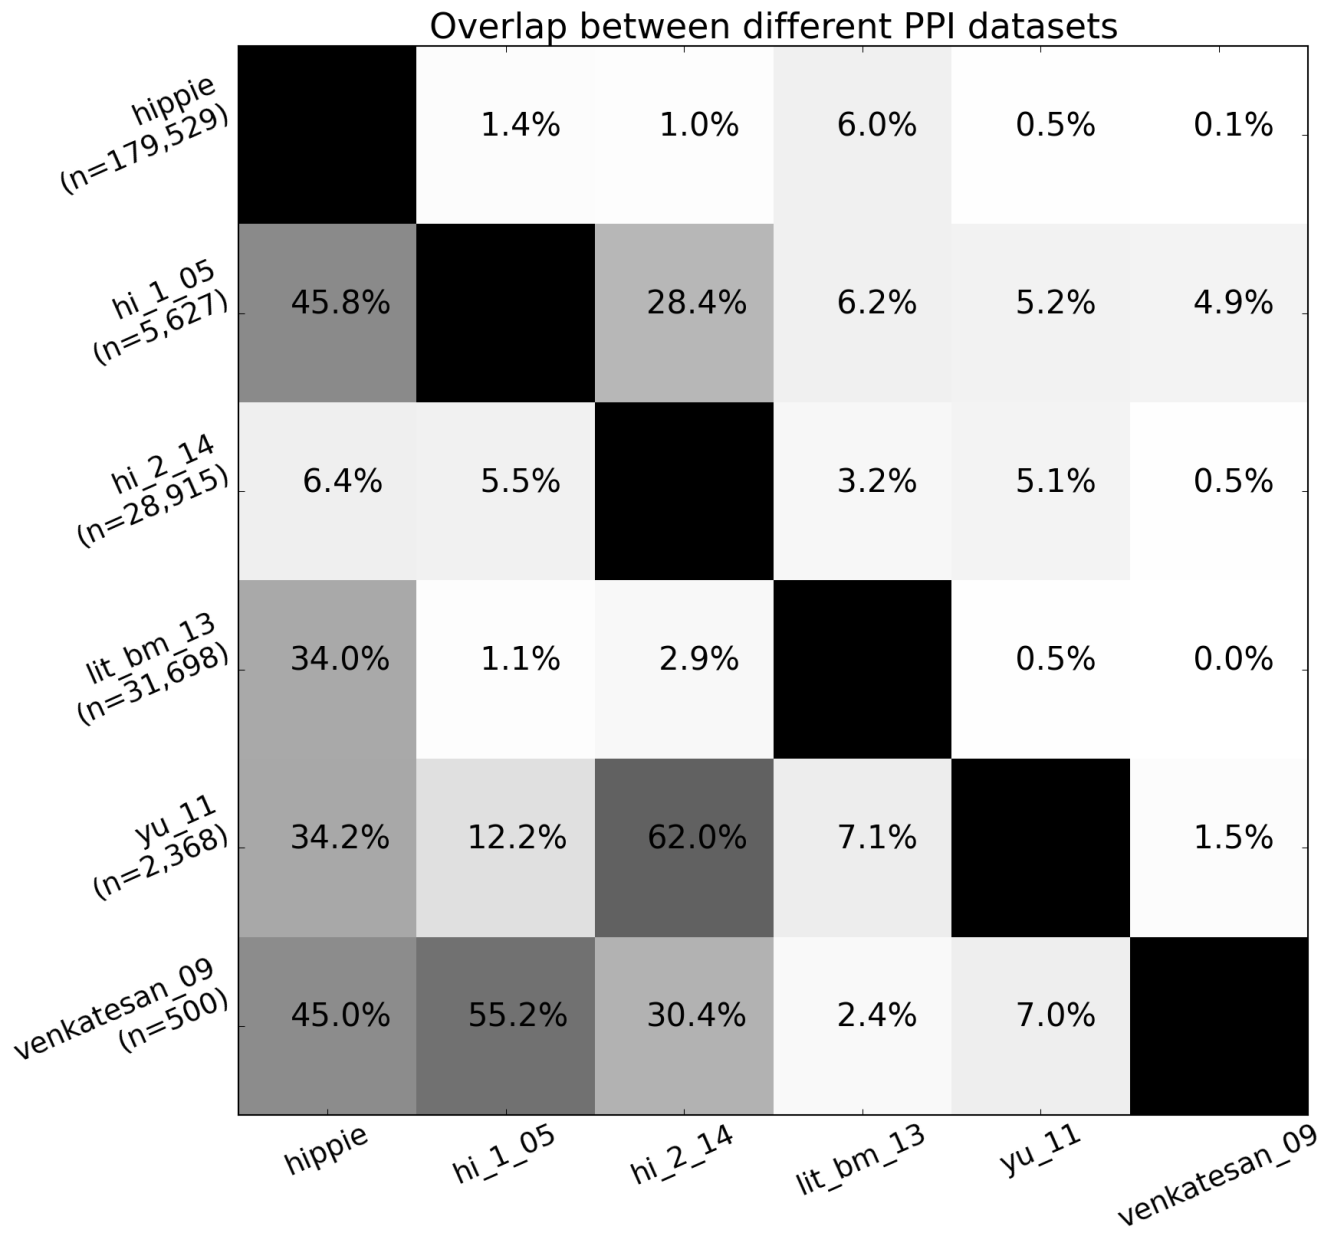
\includegraphics[width=0.6\textwidth]{static/profs/ppi_database_overlap.png}
	\caption[Overlap in protein-protein interaction databases.]{Overlap in protein-protein interaction (PPI) databases. The shade and value of each square denotes the percentage of PPIs in the database named on the y-axis that are also found in the database named on the x-axis. \textbf{hippie} is a meta-database, which integrates PPIs from many different sources \cite{schaefer_hippie:_2012}. \textbf{hi\_1\_05} contains PPIs discovered through a proteome-wide yeast two-hybrid experiment conducted by Rual \textit{et al.} \cite{rual_towards_2005}. \textbf{hi\_2\_14} contains PPIs discovered through a proteome-wide yeast two-hybrid experiment conducted by Rolland \textit{et al.} \cite{rolland_proteome-scale_2014}. \textbf{lit\_bm\_13} contains PPIs obtained from the literature and supported by multiple pieces of evidence \cite{rolland_proteome-scale_2014}. \textbf{yu\_11} contains PPIs obtained using ``stitch-seq'', which combines PCR stitching with next-generation sequencing \cite{yu_next-generation_2011}. \textbf{venkatesan\_09} corresponds to high-quality binary interactions found in repeat yeast two-hybrid assays conducted by Venkatesan \textit{et al.} \cite{venkatesan_empirical_2009}. \\
	The \textbf{hippie} database was downloaded from the Hippie website: \url{http://cbdm-01.zdv.uni-mainz.de/~mschaefer/hippie/}. All other datasets were downloaded from the Harvard Center for Cancer Systems Biology: \url{http://interactome.dfci.harvard.edu/H_sapiens/}.}
	\label{fig:ppi_database_overlap}
\end{figure}



\clearpage
\section{ELASPIC} \label{sec:elaspic}

The most widely-used program for predicting the deleteriousness of a mutation is Sorting Intolerant from Tolerant (SIFT) \cite{ng_sift:_2003}. SIFT runs PSI-Blast to create a multiple sequence alignment for the query protein, and computes a conservation score by looking at the likelihood of the wildtype and mutant amino acids occurring at a given position in the alignment. While SIFT is a well-established tool in the field, it is difficult to compile and install on a local machine. Furthermore, multiple sequence alignments constructed by SIFT can be several megabytes in size, and caching this data for an entire proteome would require a non-trivial amount of storage space.

Another popular sequence-based algorithm is Provean \cite{choi_predicting_2012}. Provean also creates a multiple sequence alignment for the query protein. However, instead of using the entire alignment, Provean runs CD-HIT to select under 50 representative sequences, referred to as the ``supporting set'', which capture the diversity of the alignment. The supporting set for a particular protein can be precalculated and stored for future use. If a supporting set is available, calculating the Provean score takes several seconds per mutation. Provean is reported to achieve similar performance to SIFT \cite{choi_predicting_2012}. However, unlike SIFT, it is freely available under the GPLv3 license, it compiles easily and it runs on all modern Linux distributions.

Many other tools have been developed that offer various advantages over SIFT / Provean. PolyPhen-2 \cite{adzhubei_predicting_2001} uses support vector machines to combine a conservation score with different sequential and structural features of the wildtype and mutant residue. However, since PolyPhen-2 is trained on a dataset of human deleterious mutations, it is difficult to use in downstream applications, as one would have to make sure to exclude the PolyPhen-2 training set throughout the training and validation process. FATHMM \cite{shihab_ranking_2014} constructs a hidden Markov model based on the alignment, and is reported to achieve marginally higher accuracy than SIFT / Provean. Other techniques offering various advantages over SIFT / Provean include MutPred \cite{li_automated_2009}, MutationAssesor \cite{network_integrated_2011}, CADD \cite{kircher_general_2014}, CONDEL \cite{gonzalez-perez_improving_2011}, and others.






The ELASPIC project was started by Niklas Berliner and others in 2014 \cite{berliner_combining_2014}. ELASPIC uses Modeller \cite{webb_comparative_2002} to construct homology models of domains and domain-domain interactions, FoldX to optimize those model and to introduce mutations \cite{schymkowitz_foldx_2005}, and the gradient boosting regressor algorithm \cite{berliner_combining_2014}, implemented in scikit-learn \cite{scikit-learn}, to combine FoldX energy scores with sequence-based and other features and predict the energetic impact of a mutation on the stability of a single domain or the affinity between two domains.

Since the original publication, ELASPIC was updated in many ways in order to make it easy to configure and run on different systems, and to make it possible to run ELASPIC on a distributed cluster as a backend to the ELASPIC webserver. Instead of using SIFT, as discussed in the original publication, we switched to using Provean, as it proved to be much easier to configure and install, and gave an option of precalculating supporting sets which could be used to calculate the Provean score for other mutations in the same protein in seconds. We switched to using MSMS instead of NACCESS for calculating solvent-accessible surface area of residues because MSMS was able to handle better misformed PDB files. We created two libraries for running selaspic

An overview of the updated ELASPIC pipeline is presented in Figure \ref{fig:elaspic_pipeline}. ELASPIC includes a Python library for construction sequence alignments, constructing Provean supporting sets and computing the Provean score, constructing homology models, running FoldX, and predicting the $\Delta \Delta G$ of the mutation. It also includes a ``Standalone Pipeline'' (Figure \ref{fig:elaspic_pipeline} right) and a ``Database Pipeline'' (Figure \ref{fig:elaspic_pipeline} left), which wrap the ELASPIC library and provide command line options for mutating local PDB files and proteins in the ELASPIC database.

The source code for the ELASPIC pipeline is hosted on GitHub (\url{https://github.com/kimlaborg/elaspic}), ELASPIC documentation is hosted on ReadtheDocs (\url{http://elaspic.readthedocs.io/}), and precalculated data can be downloaded from the ELASPIC website (\url{http://elaspic.kimlab.org/static/download/}).


\begin{figure}[!tb]
	\centering
	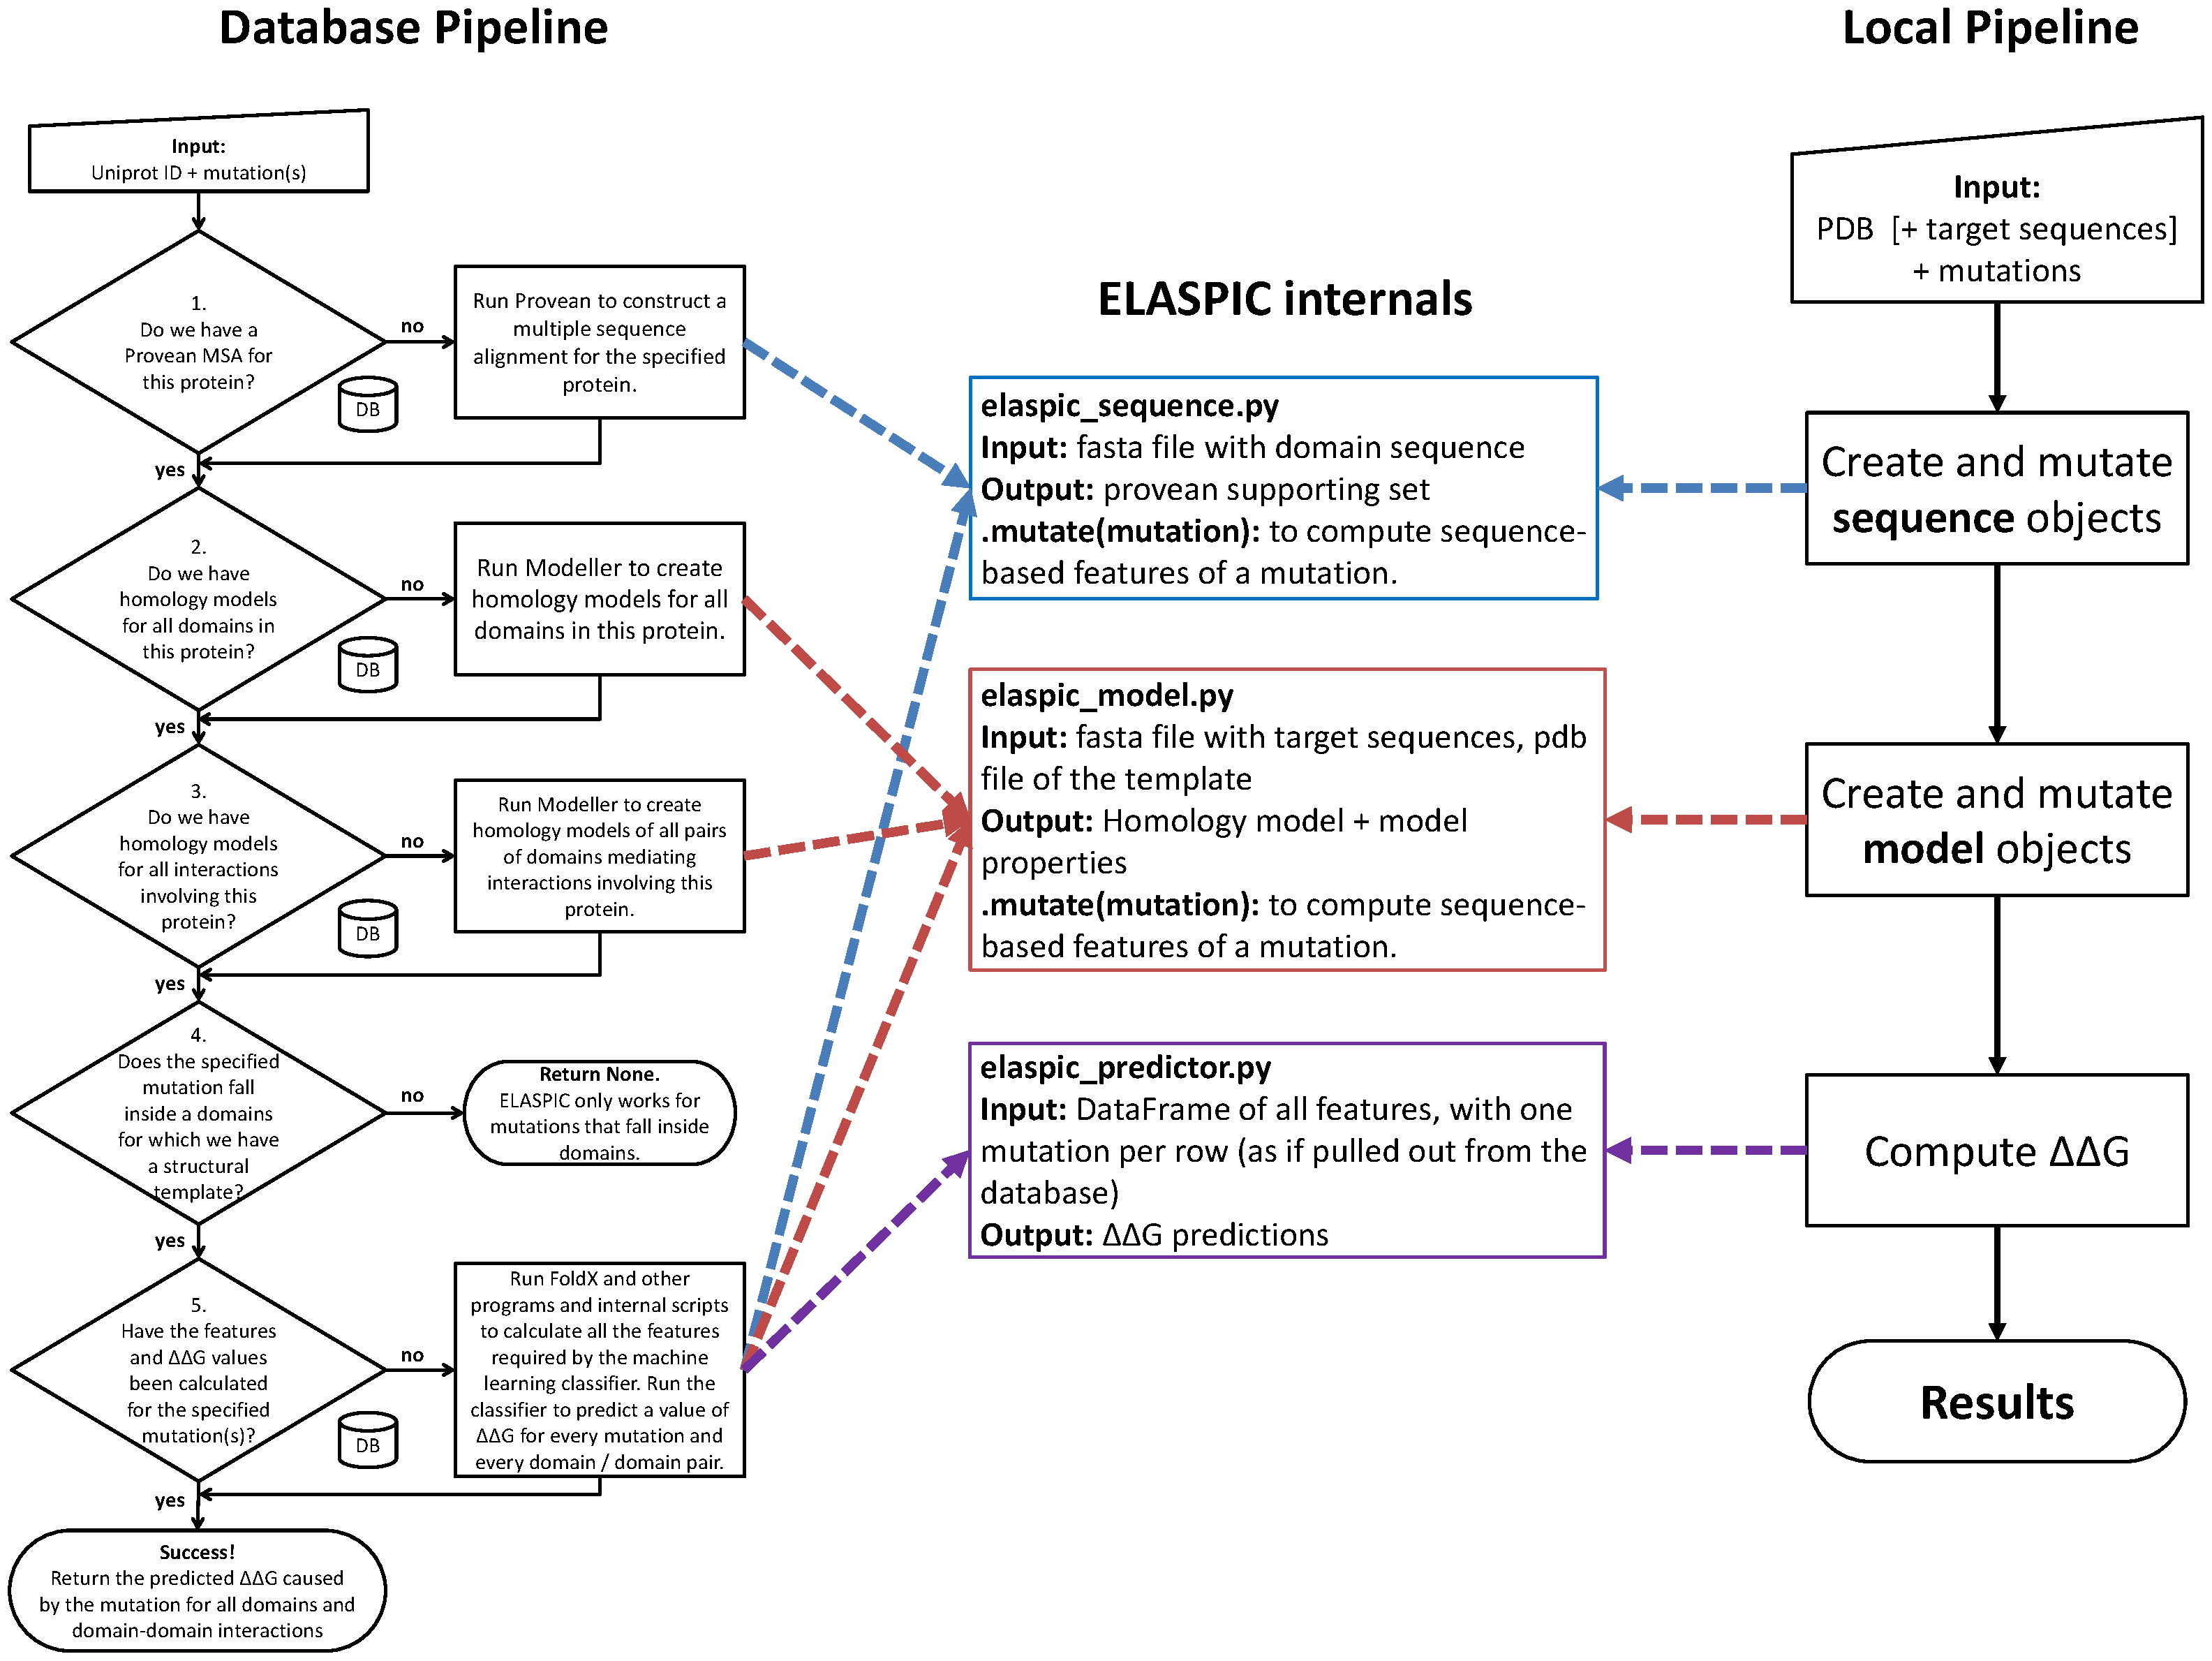
\includegraphics[width=1.0\textwidth]{static/elaspic/elaspic_flowchart.pdf}
	\caption[ELASPIC pipeline.]{Overview of the ELASPIC pipeline. \textbf{Database Pipeline:} A user runs the ELASPIC pipeline by specifying the UniProt identifier of the protein being mutated, and one or more mutations affecting that protein. At each decision node, the pipeline queries the database (Figure \ref{fig:elaspic_database_schema}) to check whether or not the required information has been calculated previously. If the required data has not been calculated, the pipeline calculates it on the fly and stores the results in the database for later retrieval. The pipeline proceeds until homology models of all domains in the protein, and all domain-domain interactions involving the protein, have been calculated, and the $\Delta \Delta G$ has been predicted for every specified mutation. \textbf{Local Pipeline:} A user runs the ELASPIC pipeline by specifying a PDB file with the structure of the protein that they wish to mutate and one or more mutations, or by specifying a FASTA file with the sequence of the protein that they wish to mutate, a PDB file with the structural template to be used for homology modelling and one or more mutations. ELASPIC runs Provean to calculate the supporting set, runs MODELLER to make the homology model, and runs FoldX to compute structural features describing the wildtype and mutant residues. Results are stored in a local \textit{.elaspic} folder and are not recalculated if the user decides to run more mutations.}
	\label{fig:elaspic_pipeline}
\end{figure}


\subsection{Standalone pipeline}

The standalone pipeline works without downloading and installing a local copy of the ELASPIC and PDB databases, but requires a PDB structure to be provided for every mutation. The output of the pipeline is saved as JSON files inside the \textit{.elaspic} subfolder created in the working directory. The general overview of the local pipleine is presented on the right side of Figure \ref{fig:elaspic_pipeline}.


\subsection{Database pipeline}

The database pipeline allows mutations to be performed on a proteome-wide scale, without having to specify a structural template for each protein. This pipeline requires a local installation of a relational database containing ELASPIC domain definitions and templates, as well as a local copy of the BLAST and PDB databases.

The general overview of the database pipleine is presented on the left side of Figure \ref{fig:elaspic_pipeline}. A user runs the ELASPIC pipeline specifying the Uniprot ID of the protein being mutated, and one or more mutations affecting that protein. At each decision node, the pipeline queries the database to check whether or not the required information has been previously calculated. If the required data has not been calculated, the pipeline calculates it on the fly and stores the results in the database for later retrieval. The pipeline proceeds until homology models of all domains in the protein, and all domain-domain interactions involving the protein, have been calculated, and the $\Delta \Delta G$ has been predicted for every specified mutation.

Results of the database pipeline are store in the ELASPIC database. An overview of the ELASPIC database schema is presented in Figure \ref{fig:elaspic_database_schema}, and a description of each database table is provided in Table \ref{tab:elaspic_database_schema}.

\begin{figure}[!tb]
	\centering
	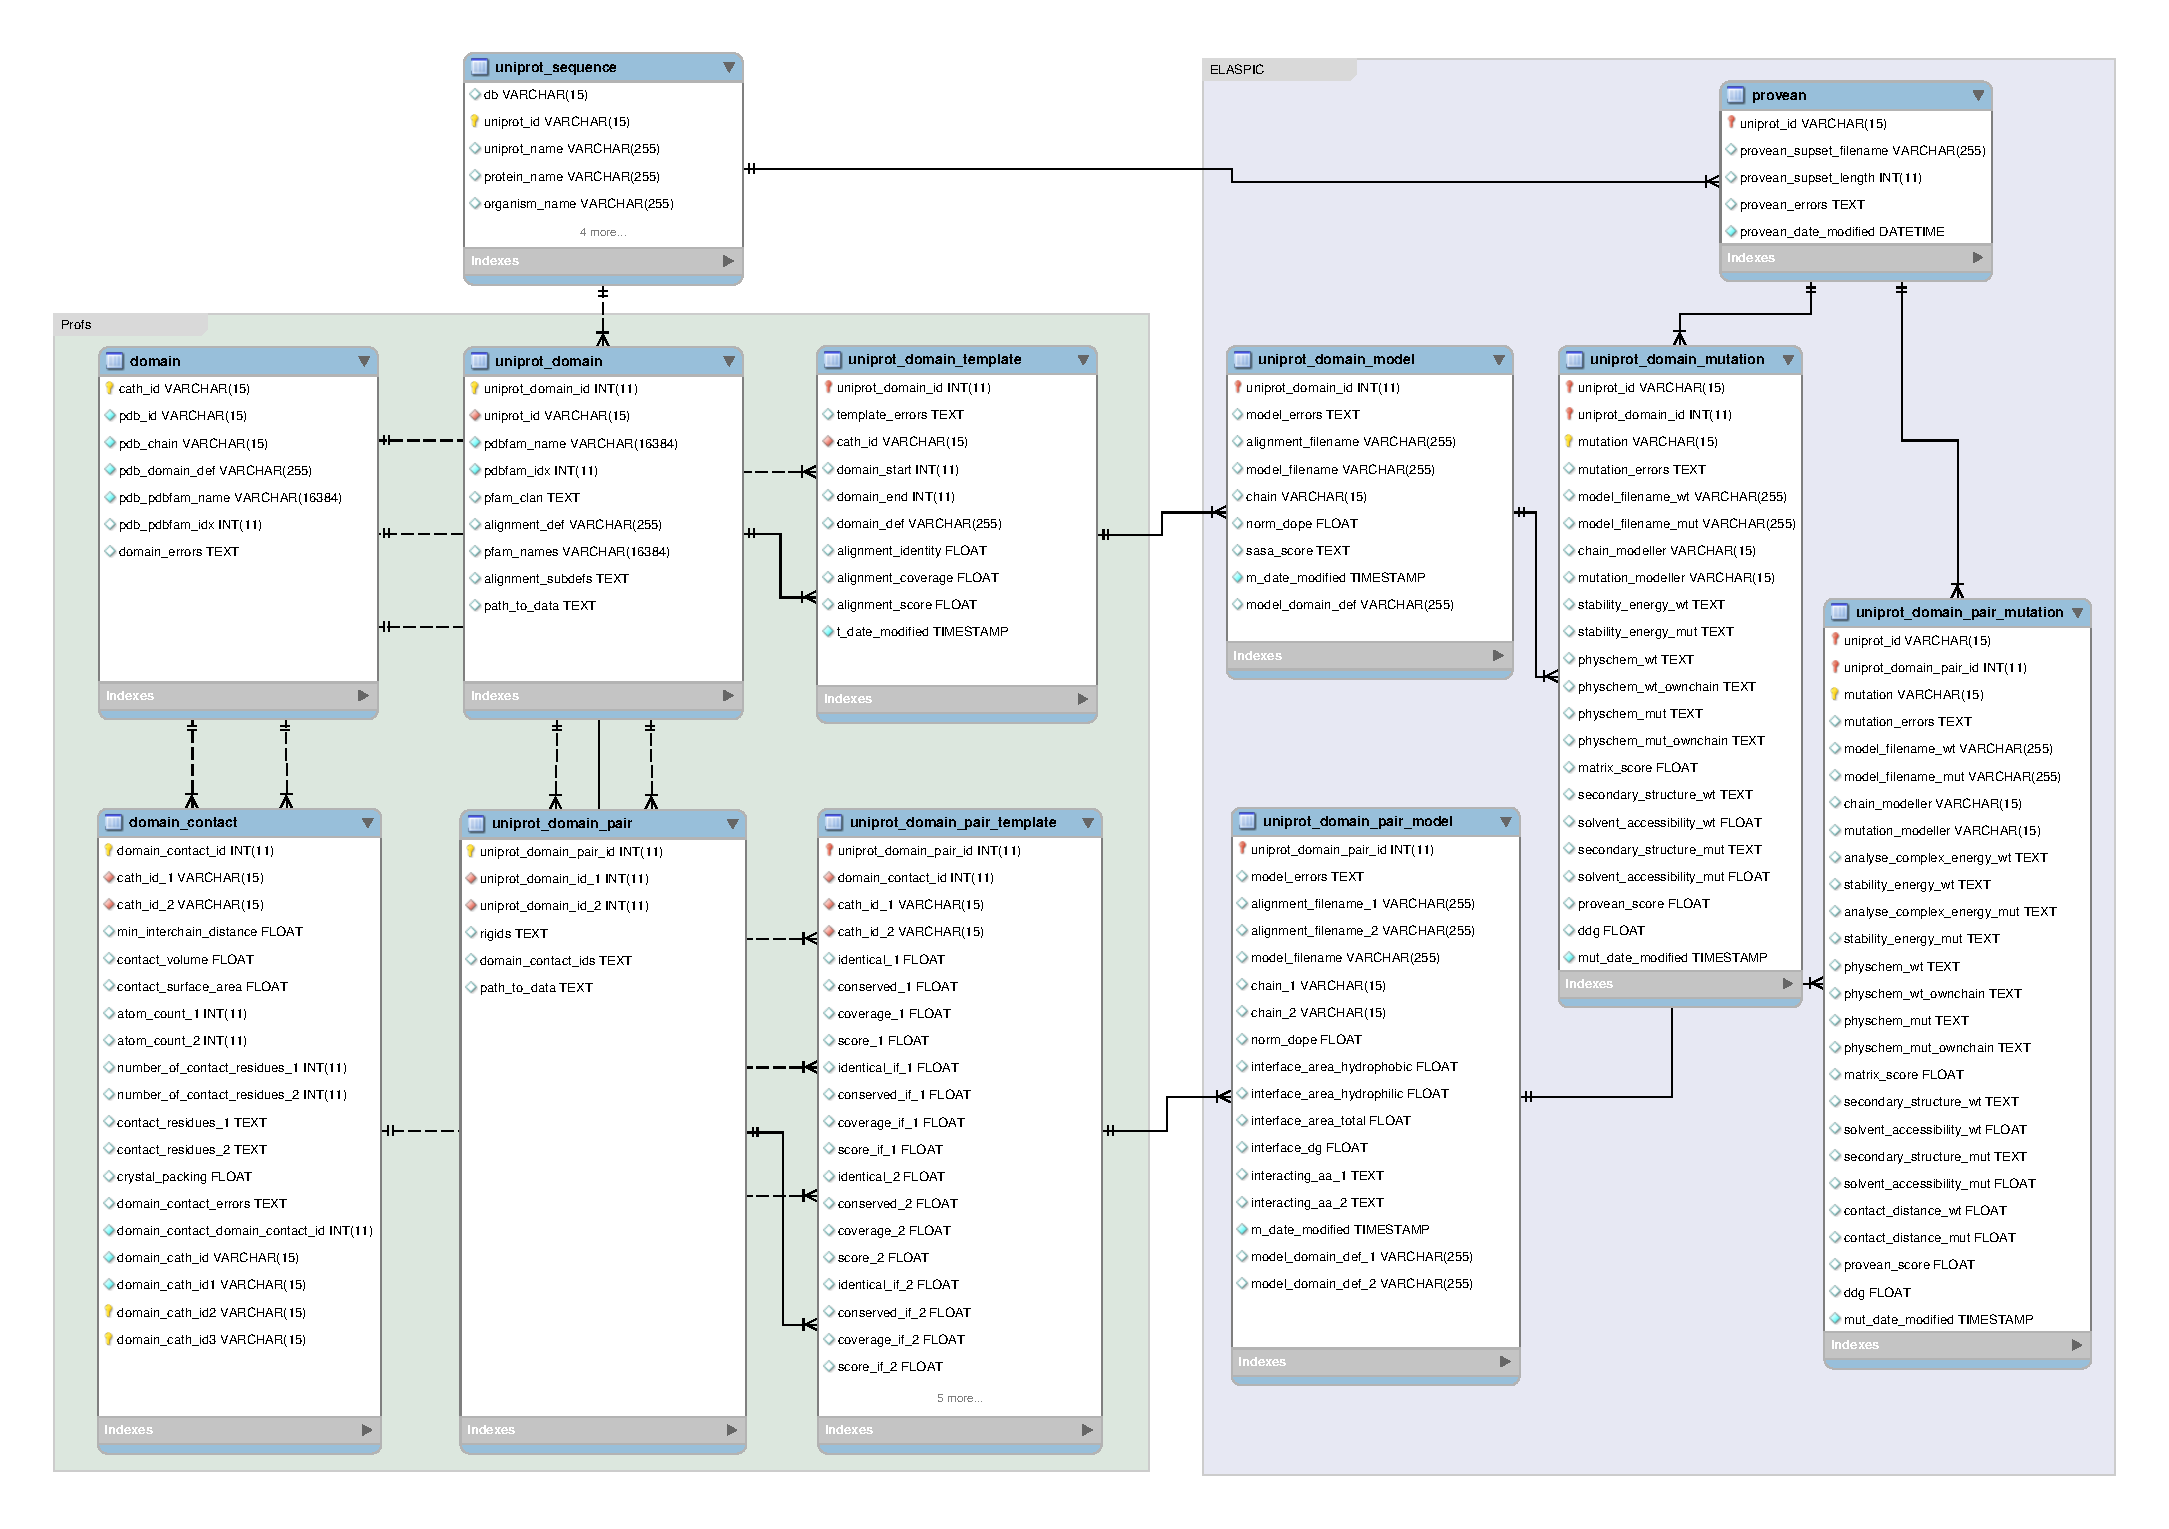
\includegraphics[width=1.0\textwidth]{static/elaspic/elaspic_schema.pdf}
	\caption[ELASPIC database schema.]{ELASPIC database schema. Tables on the green plate titled Profs are calculated using the Profs pipeline, following the procedure outlined in Figure \ref{fig:profs_pipeline}. Tables on the purple plate titled ELASPIC are calculated using the ELASPIC pipeline, following the ``database pipeline'' shown in Figure \ref{fig:elaspic_pipeline}. \\
	A detailed description of each table is provided in Table \ref{tab:elaspic_database_schema}.}
    \label{fig:elaspic_database_schema}
\end{figure}


\begin{table}[!tb]
\caption[ELASPIC database schema.]{Description of the tables in the ELASPIC database schema (Figure \ref{fig:elaspic_database_schema}).} \label{tab:elaspic_database_schema}
\begin{tabular}{l | p{10cm}}
	\toprule
	Table name & Table description \\
	\midrule
	\textbf{domain} & Contains Profs domain definitions for all proteins in the PDB. \\
	\textbf{domain\_contact} & Contains information about interactions between Profs domains in the PDB. Only interactions that are predicted to be real by NOXclass \cite{zhu_noxclass:_2006} are included in this table. \\
	\textbf{uniprot\_sequence} & Contains protein sequences for all proteins that are annotated with Profs domains in the \textbf{uniprot\_domain} table. This table is constructed by downloading and parsing \textit{uniprot\_sprot\_fasta.gz}, \textit{uniprot\_trembl\_fasta.gz} and \textit{homo\_sapiens\_variation.txt} files from the Uniprot. \\
	\textbf{provean} & Contains information about Provean \cite{choi_predicting_2012} supporting set files. The construction of a supporting set is the longest part of running Provean. Thus, in order to speed up the evaluation of mutations, the supporting set is precalculated and stored for every protein. \\
	\textbf{uniprot\_domain} & Contains Profs domain definitions for proteins in the \textbf{uniprot\_sequence} table. This table is obtained by downloading Pfam domain definitions for all known proteins from SIMAP \cite{rattei_simapcomprehensive_2010}, and mapping those proteins to Uniprot using the MD5 hash of each sequence. Overlapping and repeating domains are either merged or deleted, as described in \cite{witvliet_elaspic_2016}. \\
	\textbf{uniprot\_domain\_template} & Contains structural templates for domains in the \textbf{uniprot\_domain} table. The \textit{domain\_def} column contains expanded and corrected domain definitions for every domain. \\
	\textbf{uniprot\_domain\_model} & Contains information about the homology models that were created using structural templates in the \textbf{uniprot\_domain\_template} table. \\
	\textbf{uniprot\_domain\_mutation} & Contains information about the structural impact of core mutations, calculated by introducing those mutations into homology models listed in the \textbf{uniprot\_domain\_model} table. The \textit{ddg} column contains the predicted change in the Gibbs free energy of protein folding. \\
	\textbf{uniprot\_domain\_pair} & Contains pairs of domains that are likely to mediate the interaction between pairs of proteins listed in Hippie \cite{schaefer_hippie:_2012} and Rolland \textit{et al.} \cite{rolland_proteome-scale_2014}. \\
	\textbf{uniprot\_domain\_pair\_template} & Contains structural templates for domain pairs in the \textbf{uniprot\_domain\_pair} table. \\
	\textbf{uniprot\_domain\_pair\_model} & Contains information about homology models that were created using structural templates in the \textbf{uniprot\_domain\_pair} table. \\
	\textbf{uniprot\_domain\_pair} & Contains information about the structural impact of interface mutations, calculated by introducing those mutations into homology models listed in the \textbf{uniprot\_domain\_pair\_model} table. The \textit{ddg} column contains the predicted change in the Gibbs free energy of protein-protein binding. \\
	\bottomrule
\end{tabular}
\end{table}


\clearpage
\subsection{Jobsubmitter}

In order to make ELASPIC accessible to a wider scientific audience, Daniel Witvliet created the ELASPIC webserver, which allows users to run ELASPIC for their protein and mutation of interest and to analyze interactively ELASPIC results \cite{witvliet_elaspic_2016}.

One limitation of the webserver was that it spawned ELASPIC jobs on the same virtual machine as the webserver. This meant that only a few mutations could be analyzed at a time, and that the webserver could stall when running mutations in a protein lacking a precalculated Provean supporting set, since constructing a Provean supporting set could require more RAM than the virtual machine had available. In order to make the webserver scale to thousands of mutations, we decided to restructure the job execution backend to run ELASPIC on the local Sun Grid Engine (SGE) cluster. However, this design introduced several challenges.

First, since users can run multiple mutations affecting the same protein, we had to make sure that the Provean supporting sets and homology models are calculated first, before jobs for individual mutations are submitted to the cluster. Otherwise, each mutation would initiate the calculation of a Provean supporting set, which can require more than 5 GB of memory, and a homology model, which can take more than 30 minutes to complete. This would lead to many unnecessary jobs, drastically lowering our throughput, and could lead to inconsistent results, since different jobs can generate different supporting sets and homology models, even for the same protein, due to the inherent randomness of those tasks.

Second, jobs running on a SGE cluster can die unexpectedly, if, for example, they exceed allocated resources, or if the node on which they are executing experiences a hardware failure. In most cases, the jobs do not get an opportunity to send an error message before they are terminated. Therefore, we had to keep track of all running jobs, and resubmit jobs that do not finish successfully.

Third, in order to send a ``Job Complete'' email once all mutations submitted by a particular user have been evaluated, we had to keep track of the relationship between mutations and users that submitted those mutations.

One possible way to address those design requirements would be to use an asynchronous task queue, such as Celery. However, since different tasks inside the queue do not have a shared memory state, each task would have to periodically execute a \textit{qstat} command on the SGE master node in order to monitor the status of the submitted jobs. Since we could have thousands of mutations running on the cluster at the same time, this would not be a scalable solution.

An alternative approach, which we used for the final design, was to create an independent web service responsible for submitting ELASPIC jobs to the SGE cluster and monitoring their progress. We called this web service the ELASPIC ``jobsubmitter''. It was implemented using the \textit{aiohttp} library, which leverages the \textit{asyncio} event loop and improved support for asyncronous programming present in Python 3.5 (Figure \ref{fig:elaspic_jobsubmitter}). Once the jobsubmitter receives a \textit{GET} or \textit{POST} request containing a set of mutations, information concerning those mutations is distributed into the following queues:

\vspace{-\topsep}
\begin{itemize}
	\itemsep0em
	\item A ``Provean'' queue, which contains proteins for which a Provean supporting set has not been calculated.
	\item A ``homology model'' queue, which contains proteins for which a homology model has not been calculated.
	\item A ``mutation'' queue, which contains individual mutations.
	\item An ``email'' queue, which contains the set of mutations associated with each job.
\end{itemize}

The information from those queues is then processed by the corresponding coroutines:

\vspace{-\topsep}
\begin{itemize}
	\itemsep0em
	\item For each protein in the ``Provean'' queue, a job is submitted to the SGE cluster, which calculates the Provean supporting set. If the Provean supporting set for the protein has already been calculated, the protein is taken of the ``Provean'' queue with no further action.
	\item For each protein in the ``homology model'' queue, a job is submitted to the SGE cluster, which calculates the homology model of the protein. If the homology model of the protein has already been calculated, the protein is taken of the ``homology model'' queue with no further action.
	\item For each mutation in the ``mutation'' queue, a job is submitted to the SGE cluster, which runs ELASPIC to calculate the $\Delta \Delta G$ of the mutation. This happens \textit{only if the Provean supporting set and homology model for the protein have already been calculated!}
	\item For each job in the ``email'' queue, a ``Job Complete'' email is sent to the specified email address once all mutations for the associated job have been completed.
\end{itemize}

The ELASPIC jobsubmitter is highly performant. It is able to handle over 150 requests per second, even with 30,000 mutations already being processed by the web service (Figure \ref{fig:elaspic_jobsubmitter_performance}).

\begin{figure}[!htb]
	\centering

	\begin{subfigure}{0.8\textwidth}
		\centering
		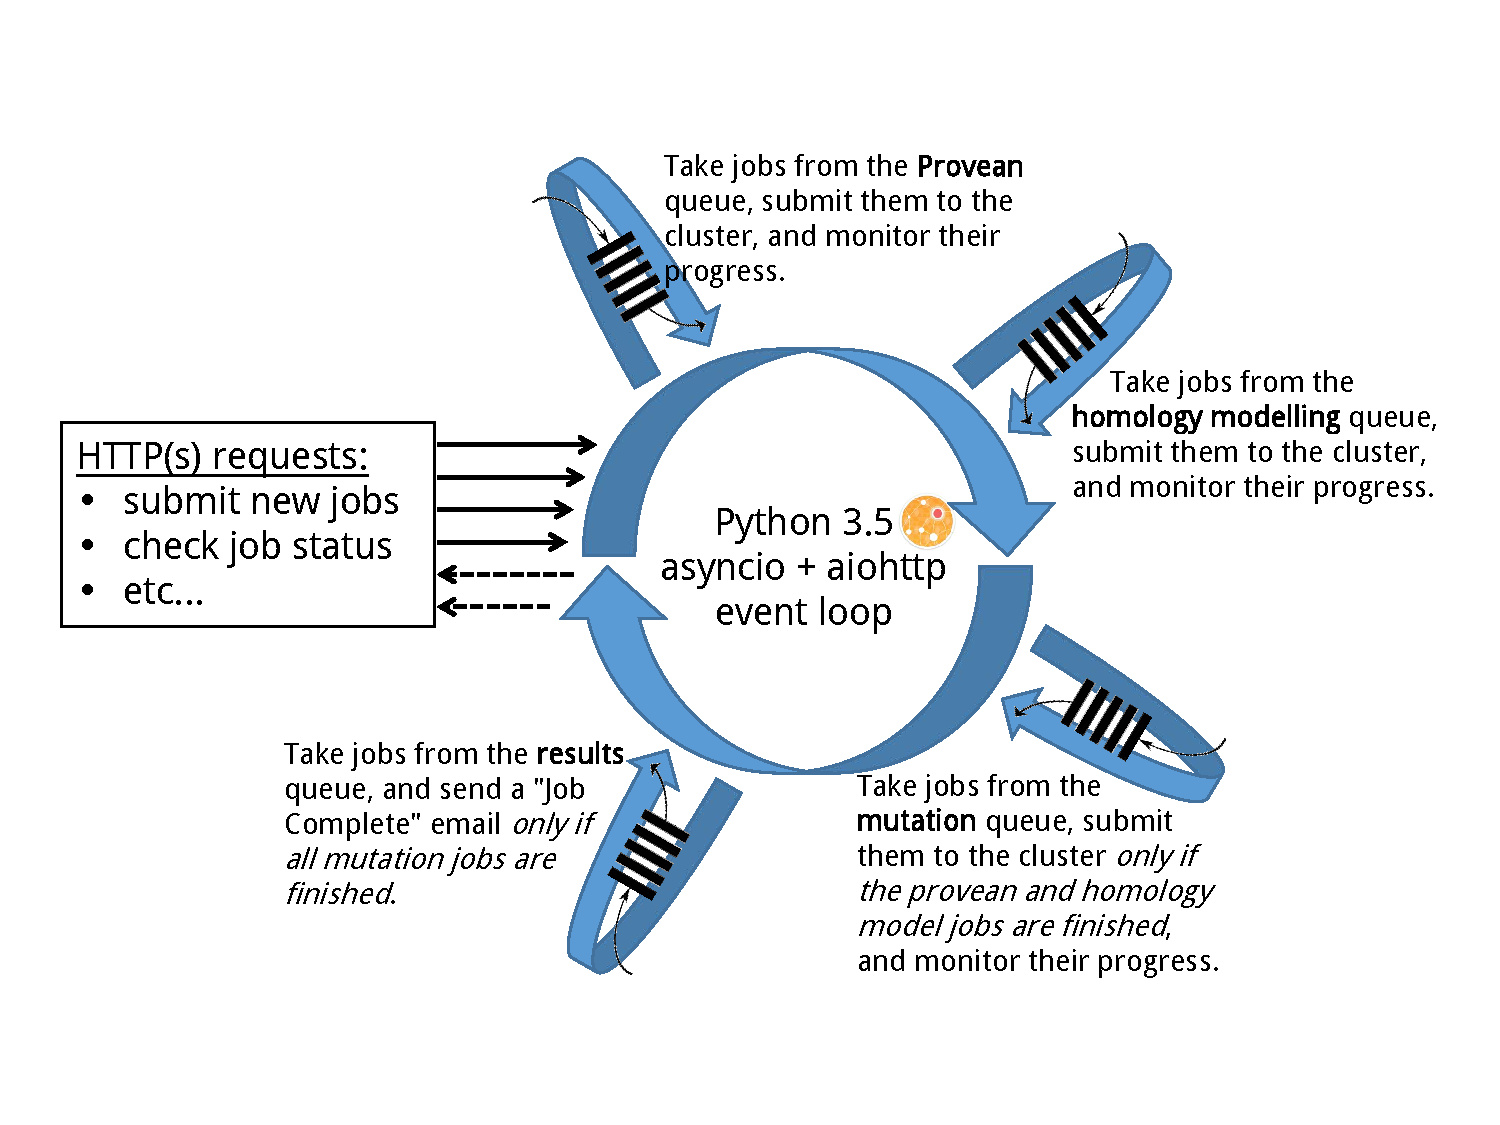
\includegraphics[width=1\linewidth]{static/elaspic/elaspic_jobsubmitter.pdf}
		\caption{Overview of the ``jobsubmitter'' web service. The web service was implemented using Python 3.5 and the \textit{aiohttp} library. It contains a central \textit{asyncio} event loop, data structures holding information about the mutations being processed, and coroutines which submit jobs to the SGE cluster, monitor job progress, and perform other maintenance tasks.}
		\label{fig:elaspic_jobsubmitter}
	\end{subfigure}
	\vspace*{10mm}

	\begin{subfigure}[t]{0.8\textwidth}
		\centering
		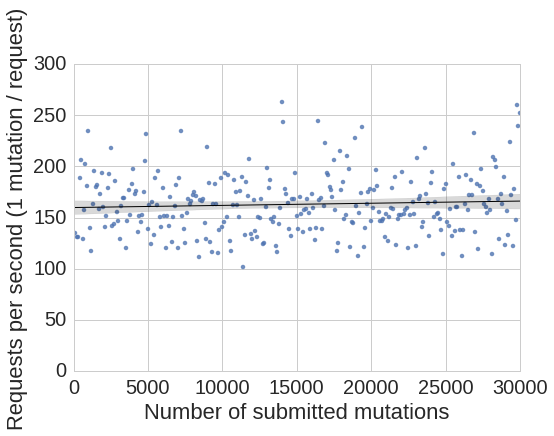
\includegraphics[width=0.7\linewidth]{static/elaspic/elaspic_jobsubmitter_performance.png}
		\caption{Plot showing the number of requests per second handled by the ELASPIC jobsubmitter as a function of the number of mutations that are already being processed.}
		\label{fig:elaspic_jobsubmitter_performance}
	\end{subfigure}
	\vspace*{5mm}

	\caption[ELASPIC jobsubmitter.]{
	Implementation (a) and performance (b) of the ELASPIC ``jobsubmitter''.
	}
	\label{fig:ELASPIC jobsubmitter}

\end{figure}



\clearpage
\subsection{Precalculated data}

In order to increase the speed with which the ELASPIC webserver could generate results, we attempted to precalculate homology models and Provean supporting sets for all human proteins, and to calculate mutations known to be involved in human disease.

Out of 20,270 proteins in human SwissProt, 18,355 proteins have at least one Pfam domain, and 14,015 proteins have a Pfam domain for which we could find a structural template in the PDB (Figure \ref{fig:protein_statistics}). We could create a homology model of at least one domain in 13,796 proteins, with the fraction of each protein covered by a homology model shown in Figure \ref{fig:structural_coverage_hist}. On the domain level, out of a total of 38,243 domains with a structural template, we could create a homology model for only 29,201 domains, or 76\% (Figure \ref{fig:domain_statistics}). The main reason for failing to calculate a homology model was low sequence identity between the domain being modelled and the structural template.

We also attempted to create a homology model for all protein pairs found in the HIPPIE \cite{schaefer_hippie:_2012} and CCSB \cite{rolland_proteome-scale_2014} databases, keeping only the pairs where each protein has at least one domain with a homology model and where we would could find a structural template of the protein-protein interaction. Out of a total of 19,964 such protein pairs, we calculated a homology models for 18,956, or 95 \% (Figure \ref{fig:elaspic_precalculated_interface}).

We successfully precalculated a Provean supporting set for all 14,015 human proteins with a Profs domain with a structural template. We also ran ELASPIC for over 990,000 million mutations implicated in human diseases or found in human cancers, including nearly 600,000 mutations in different protein-protein interfaces.


\begin{figure}[!tb]
	\centering

	\begin{subfigure}[t]{0.48\textwidth}
		\centering
		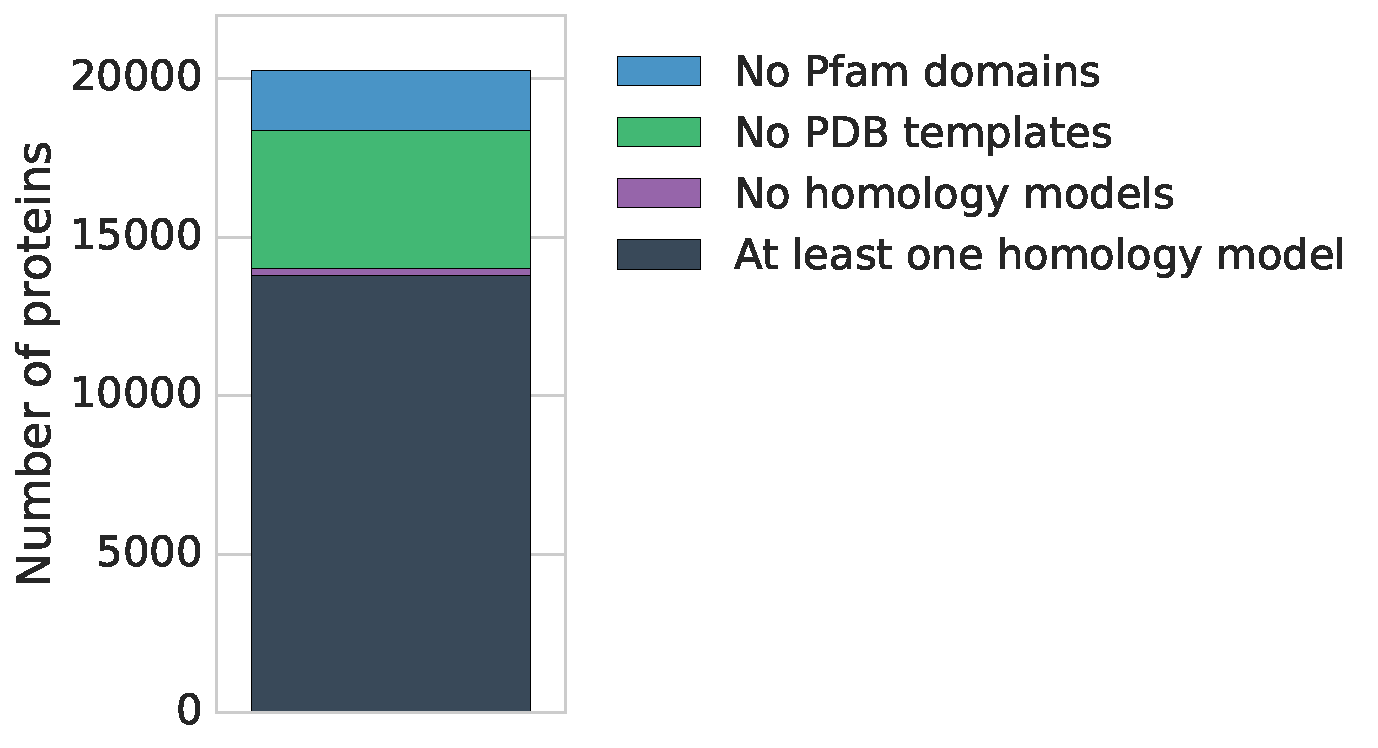
\includegraphics[width=1\linewidth]{static/elaspic_training_set/elaspic_statistics/protein_statistics.pdf}
		\caption{Diagram showing the number of \textit{proteins} in the human SwissProt database that have no Pfam domains (blue), that have Pfam domains but no structural templates (green), that have Pfam domains and structural templates but no homology models (purple), and proteins with a homology model of at least one domain (grey).}
		\label{fig:protein_statistics}
	\end{subfigure}%
	\hspace*{5mm}
	\begin{subfigure}[t]{0.48\textwidth}
		\centering
		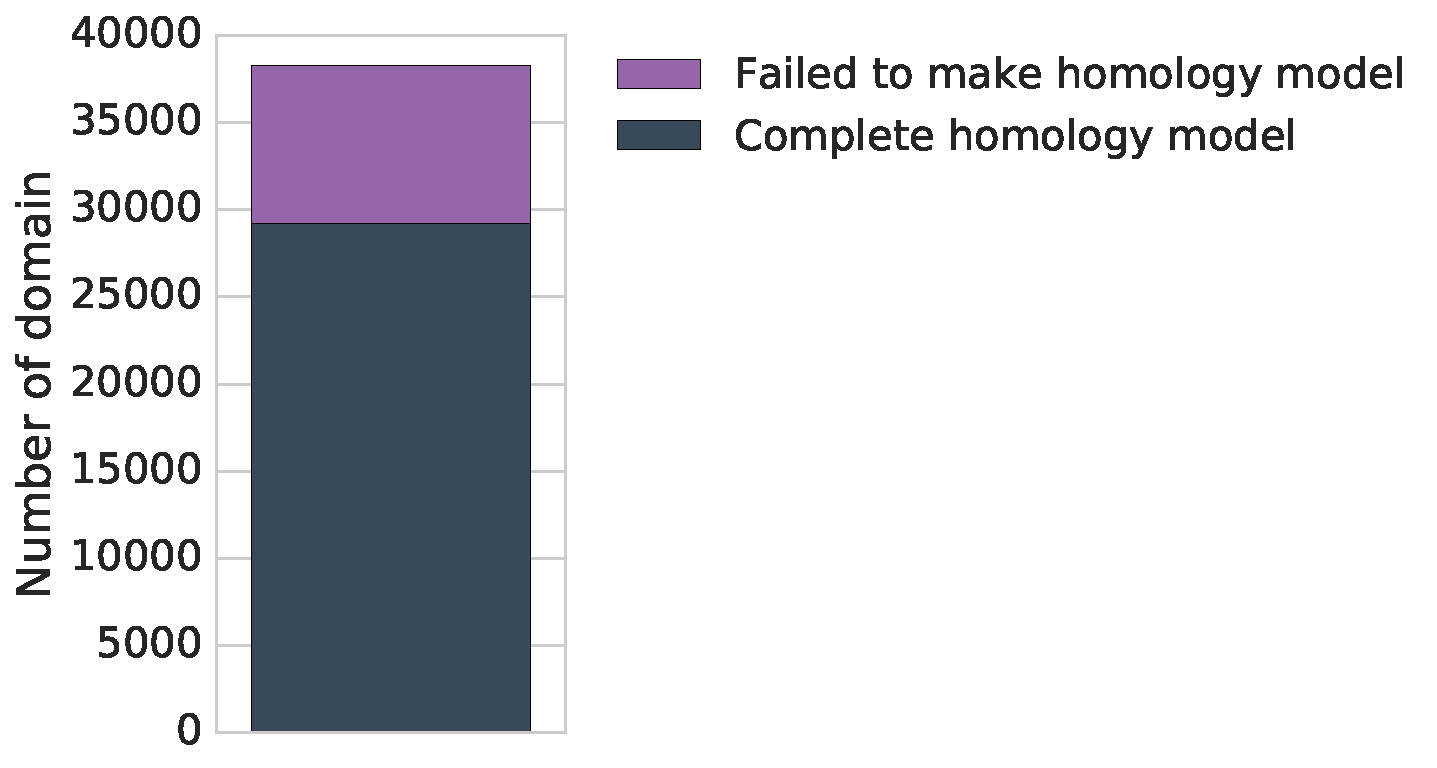
\includegraphics[width=1\linewidth]{static/elaspic_training_set/elaspic_statistics/domain_statistics.pdf}
		\caption{Diagram showing the number of \textit{domains} in all proteins in the human SwissProt database for which we failed to create a homology model (purple) and for which we successfully created a homology model (grey). The most common reason for failing to create a homology model was low sequence identity between the Profs domain and the structural template.}
		\label{fig:domain_statistics}
	\end{subfigure}
	\vspace*{10mm}

	\begin{subfigure}{0.55\textwidth}
		\centering
		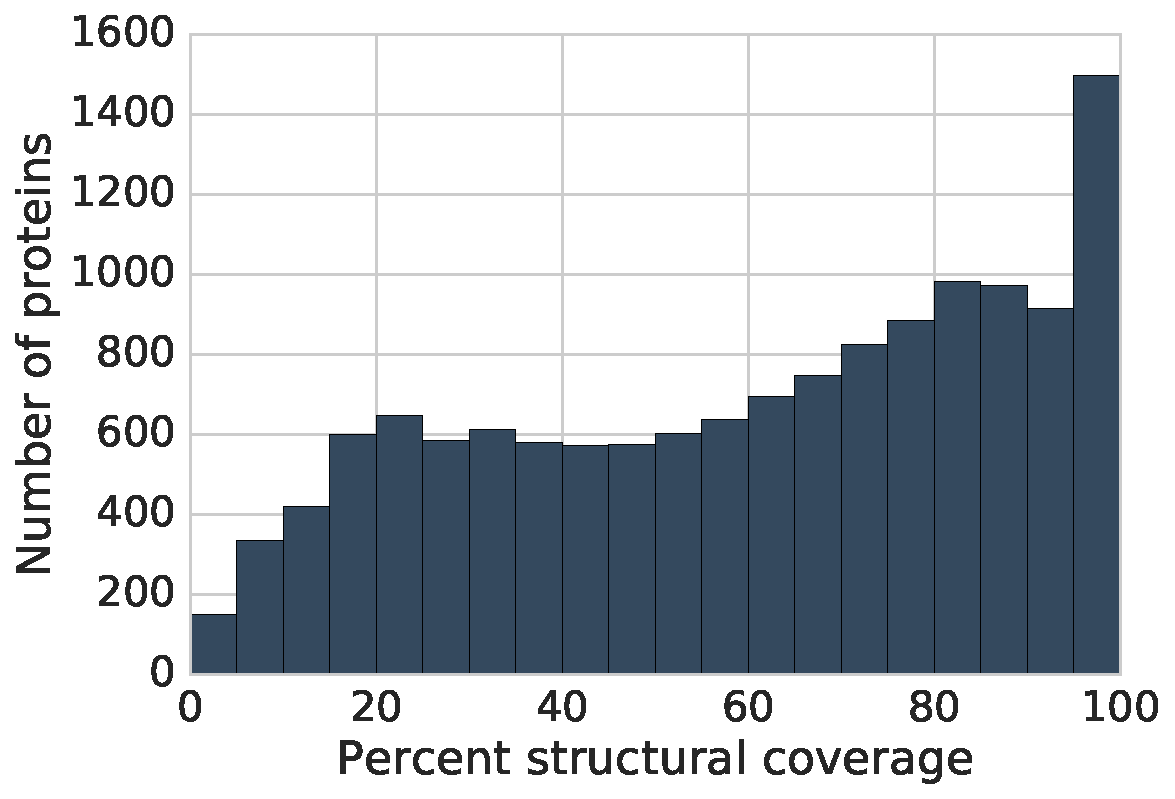
\includegraphics[width=1\linewidth]{static/elaspic_training_set/elaspic_statistics/structural_coverage_hist.pdf}
		\caption{The percentage of protein sequence covered by Profs domains with homology models, for all proteins in the human SwissProt database that have a homology model of at least one domain.}
		\label{fig:structural_coverage_hist}
	\end{subfigure}
	\vspace*{5mm}

	\caption[Precalculated homology models of human proteins.]{Plots showing the number of proteins for which we could create a homology model (a), the number of domains for which we could create a homology model (b), and the structural coverage of proteins with at least one modelled domain (c). Plots were generated using all human proteins in the SwissProt database.}
	\label{fig:elaspic_precalculated_core}
\end{figure}


\begin{figure}[!tb]
	\centering
	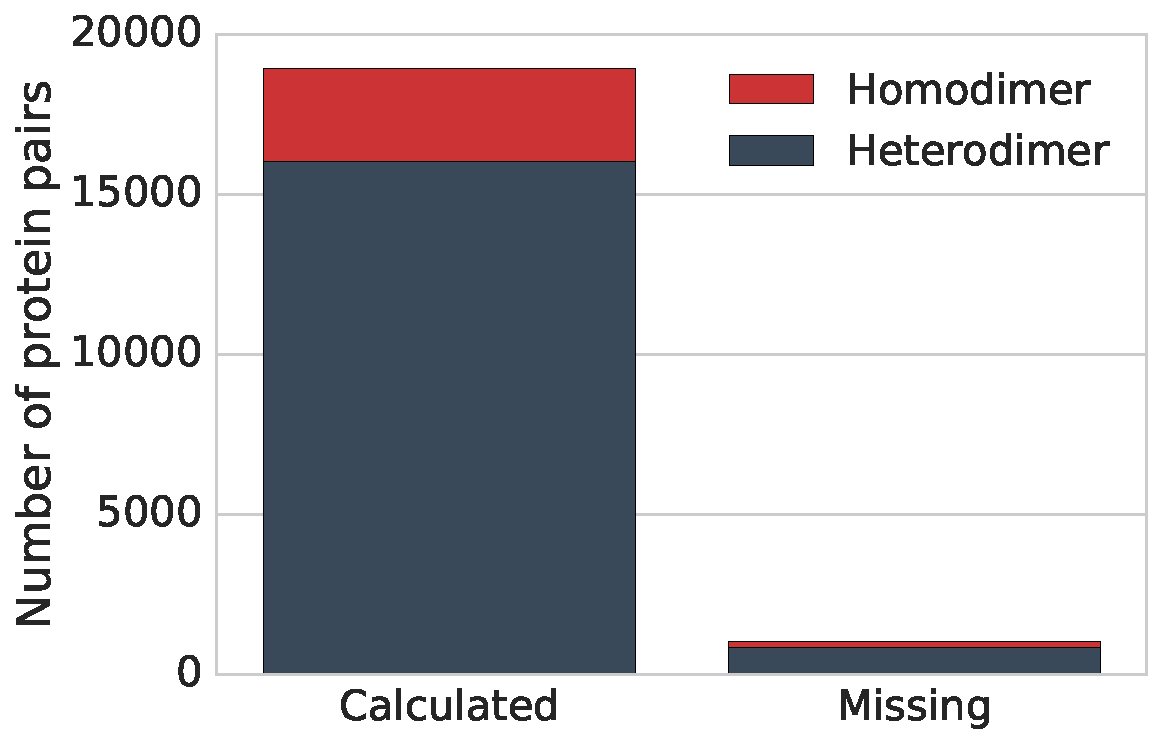
\includegraphics[width=0.5\linewidth]{static/elaspic_training_set/elaspic_statistics/missing_model_protein_pair_novarsplice.pdf}
	\caption[Precalculated homology models of human protein-protein interactions.]{Number of homo-dimeric (red) and hetero-dimeric (grey) protein-protein interactions for which we created a homology model (left) and failed to create a homology model (right). In this figure, protein-protein interactions are defined as all pairs of proteins from the human SwissProt database that are found to interact according to one of the protein-protein interaction databases (see Figure \ref{fig:ppi_database_overlap}) and that have at least one structural template of the interaction.}
	\label{fig:elaspic_precalculated_interface}
\end{figure}
